\chapter{Taylor-Approximation von Funktionen}\label{ch:Taylor}

\section{Motivation und Intuition}
Wir wollen später im \cref{ch:Dynamik} Methoden entwickeln, um Annäherungen (Approximationen) an die wahren Lösungen von Differentialgleichungen Schritt für Schritt zu berechnen. Damit ist es naheliegend, zunächst mal Methoden zur Approximation von Funktionen zu studieren (Lösungen von Differentialgleichungen sind schliesslich ebenfalls Funktionen). In diesem Kapitel werden wir die sehr wichtige und berühmte Taylor-Approximation von Funktionen kennenlernen.

Für \cref{fig:Taylor1} haben wir eine beliebige Funktion $f$ gewählt und dargestellt. Wir wollen eine Approximation von $f$ in der näheren Umgebung der Stelle $x_0 = -1$ finden. Wir können hoffen, dass sich $f$ in der Nähe von $x_0 = -1$ einigermassen gut durch die Tangente an $f$ durch den Punkt $(x_0, f(x_0)$ approximieren lässt. Diese Tangente haben wir in \cref{fig:Taylor1} eingezeichnet.

Fall die Ableitung der Funktion $f$ an der Stelle $x_0$ existiert, so lautet die Funktionsgleichung der Tangente $t$ an $f$ durch den Punkt $(x_0, f(x_0))$:
\begin{align*}
  t(x) = f(x_0) + f'(x_0)(x-x_0).
\end{align*}

Beachte, dass an der Stelle $x_0$ die Tangente den Wert $f(x_0)$ annimmt und (zumindest) dort somit exakt mit dem wahren Funktionswert übereinstimmt.

\begin{figure}[H]
  \begin{center}
    \begin{tikzpicture}
      \begin{axis}[
          axis lines = middle,
          xlabel = $x$,
          ylabel = $y$,
          domain=-6.4:2.6,
          samples=100,
          xmin=-6, xmax=2.2,
          ymin=-60, ymax=90,
          grid=both,
          xtick={-6, -5, -1, 1, 2},
          legend style={at={(1.03,0.5)}, anchor=west}
        ]
        % Plot the function f(x)
        \addplot [thick, blue] {7 + 0.3*x^1 + 0.7*x^2 + 3*x^3 + 0.5*x^4};
        \addlegendentry{$f$}

        % Draw a point at x = -1
        \addplot [only marks, mark=*, red] coordinates {(-1, 4.9)};
        % \addlegendentry{quadratische Approx.}
        \addlegendentry{\enquote{Entwicklungsstelle} $x_0 = -1$}

        % Draw the tangent line at x = -1
        \addplot [thick, dashed, red] {5.9*(x + 1) + 4.9};
        \addlegendentry{lineare Approx.}        % Plot the function f(x)
      \end{axis}
    \end{tikzpicture}
  \end{center}
  \caption{Approximation einer Funktion $f$ in der Nähe von $x_0 = -1$ mithilfe der Tangente an $f$ durch den Punkt $(x_0, f(x_0))$}\label{fig:Taylor1}
\end{figure}

\begin{myexercise}
  Gegeben sei die Funktion $f(x) = e^{2x}$. Wie lautet die Funktionsgleichung der Tangente an $f$ durch den Punkt $(3, f(3))$? Skizziere die Situation.
\end{myexercise}

Wir haben also eine Funktion $f$ lokal durch eine (affin) lineare Funktion (Tangente) der Form
\begin{align*}
  b_0 + b_1(x-x_0)
\end{align*}
approximiert. Dabei sind $b_0$ und $b_1$ irgendwelche (reelle) Konstanten (Koeffizienten). 

\emoji{light-bulb} Warum sollten wir uns jedoch auf lineare Terme Beschränken? Wir könnten doch versuchen $f$ lokal durch einen quadratischen Term der Form
\begin{align*}
  b_0 + b_1(x-x_0) + b_2(x-x_0)^2
\end{align*}
zu approximieren, wobei auch hier $b_0, b_1$ und $b_2$ Konstanten (Koeffizienten) sind. Dabei gibt $b_0$ intuitiv an, wie stark der konstante Anteil ist, $b_1$ wie stark der lineare Anteil ist und $b_2$ wie stark der quadratische Anteil ist.   

% \begin{myexercise}
%   Warum machen wir es so kompliziert und suchen eine Approximation der Form \[b_0 + b_1(x-x_0) + b_2(x-x_0)^2\] und nicht eine der (simpleren) Form \[c_0 + c_1x + c_2x^2?\] Welche wünschenswerte Eigenschaft hat die Form $b_0 + b_1(x-x_0) + b_2(x-x_0)^2$?
% \end{myexercise}

Zum jetzigen Zeitpunkt ist völlig unklar, wie die Koeffizienten $b_0, b_1$ und $b_2$ gewählt werden sollten, um eine möglichst gute Approximation zu finden. Mit der Wahl dieser Koeffizienten gemäss Taylor (wie wir bald sehen werden) erhalten wir das Szenario in \cref{fig:Taylor2}.   

\section{Idee von Taylor}

\begin{figure}[H]
  \begin{center}
    \begin{tikzpicture}
      \begin{axis}[
          axis lines = middle,
          xlabel = $x$,
          ylabel = $y$,
          domain=-6.4:2.6,
          samples=100,
          xmin=-6, xmax=2.2,
          ymin=-60, ymax=90,
          grid=both,
          xtick={-6, -5, -1, 1, 2},
          legend style={at={(1.03,0.5)}, anchor=west}
        ]

        % Plot the function f(x)
        \addplot [thick, blue] {7 + 0.3*x^1 + 0.7*x^2 + 3*x^3 + 0.5*x^4};
        \addlegendentry{$f$}

        % Draw a point at x = -1
        \addplot [only marks, mark=*, red] coordinates {(-1, 4.9)};
        % \addlegendentry{quadratische Approx.}
        \addlegendentry{\enquote{Entwicklungsstelle} $x_0 = -1$}

        % Draw the tangent line at x = -1
        \addplot [thick, dashed, red] {-10.6/2*(x+1)^2 + 5.9*(x + 1) + 4.9};
        \addlegendentry{quadratische Approx.}
      \end{axis}
    \end{tikzpicture}
  \end{center}
  \caption{quadratische Approximation von $f$ durch an der \enquote{Entwicklungsstelle} $x_0 = -1$}\label{fig:Taylor2}
\end{figure}




\clearpage
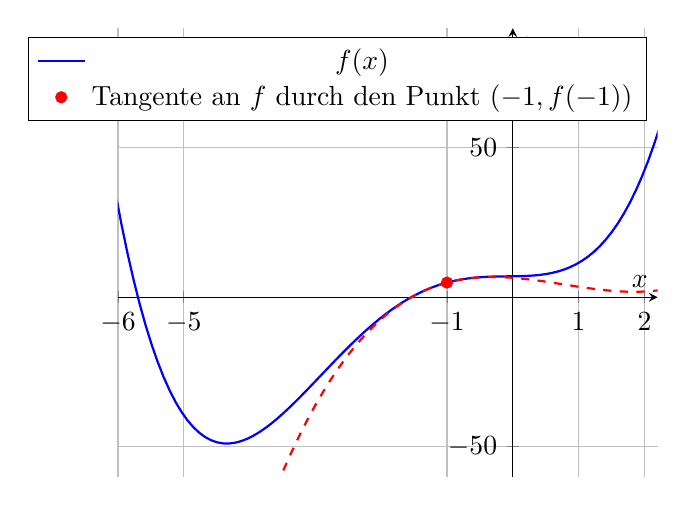
\begin{tikzpicture}
  \begin{axis}[
      axis lines = middle,
      xlabel = $x$,
      ylabel = $y$,
      domain=-6.4:2.6,
      samples=100,
      xmin=-6, xmax=2.2,
      ymin=-60, ymax=90,
      grid=both,
      xtick={-6, -5, -1, 1, 2}
    ]

    % Plot the function f(x) = x^2
    \addplot [thick, blue] {7 + 0.3*x^1 + 0.7*x^2 + 3*x^3 + 0.5*x^4};
    \addlegendentry{$f(x)$}

    % Draw a point at x = 1
    \addplot [only marks, mark=*, red] coordinates {(-1, 4.9)};
    % \addlegendentry{Point of Tangency}

    % Draw the tangent line at x = 1
    \addplot [thick, dashed, red] {6/6*(x+1)^3 - 10.6/2*(x+1)^2 + 5.9*(x + 1) + 4.9};
    \addlegendentry{Tangente an $f$ durch den Punkt $(-1, f(-1))$}

  \end{axis}
\end{tikzpicture}

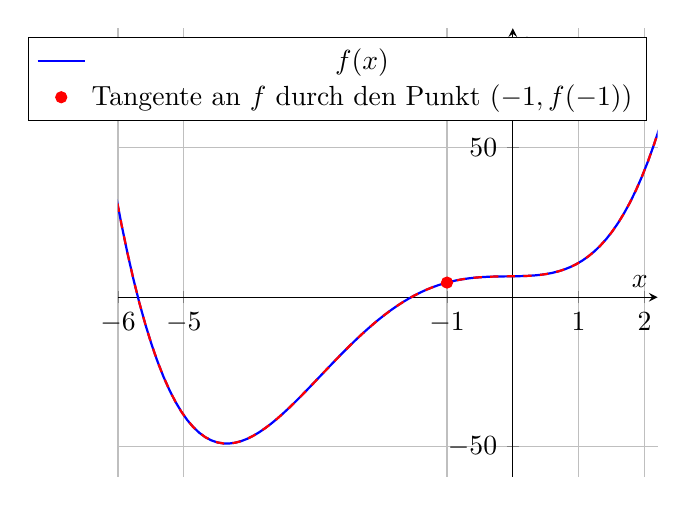
\begin{tikzpicture}
  \begin{axis}[
      axis lines = middle,
      xlabel = $x$,
      ylabel = $y$,
      domain=-6.4:2.6,
      samples=100,
      xmin=-6, xmax=2.2,
      ymin=-60, ymax=90,
      grid=both,
      xtick={-6, -5, -1, 1, 2}
    ]

    % Plot the function f(x) = x^2
    \addplot [thick, blue] {7 + 0.3*x^1 + 0.7*x^2 + 3*x^3 + 0.5*x^4};
    \addlegendentry{$f(x)$}

    % Draw a point at x = 1
    \addplot [only marks, mark=*, red] coordinates {(-1, 4.9)};
    % \addlegendentry{Point of Tangency}

    % Draw the tangent line at x = 1
    \addplot [thick, dashed, red] {12/24*(x+1)^4 + 6/6*(x+1)^3 - 10.6/2*(x+1)^2 + 5.9*(x + 1) + 4.9};
    \addlegendentry{Tangente an $f$ durch den Punkt $(-1, f(-1))$}

  \end{axis}
\end{tikzpicture}
